\documentclass{article}
\usepackage{geometry}
\usepackage{graphicx}
\usepackage{hyperref}
\usepackage{tikz}
\graphicspath{{./}}
\geometry{a4paper, portrait, margin = 1in}
\title{Introduction to Artificial Intelligence}
\date{\today}
\author{Aniruddh K Budhgavi \\ Enigma, IIITB}
\begin{document}
    \maketitle

    \section{Introduction}
        \textbf{Artificial intelligence} is a collection of methods and models
        used to mimic natural intelligence in order to perform certain tasks.
        A key feature of artificial intelligence techniques is that instead of
        the decisions being explicitly programmed, an artificial intelligence 
        system can learn from labeled or unlabeled data or from the 
        environment it works in (of course, there are exceptions to this).

        Sometimes, when talking about artificial intelligence, people instead mean
        \textbf{artificial general intelligence}, which relates to an intelligence
        which can understand and learn any cognitive task that a human can.
        Right now, AGI is the stuff of science fiction (so you can stop worrying
        about the Terminator!). In contrast, any current AI system is geared towards
        a very specific task and typically cannot generalise to different tasks.
        Even so, AI is very useful and holds much promise for 
        the present and for the future.

    \section{Examples}
        \begin{itemize}
            \item \textbf{Handwritten Digit Recognition}
                \begin{figure}[h]
                    \includegraphics[width = \textwidth]{Recognition.png}
                    \caption{A convolutional neural network. Taken from \href{https://towardsdatascience.com/mnist-handwritten-digits-classification-using-a-convolutional-neural-network-cnn-af5fafbc35e9}{towardsdatascience.com}}
                \end{figure}
            
            \clearpage
            
            \item \textbf{Object Detection}
                
                \begin{figure}[h]
                    \includegraphics[width = \textwidth]{yolo.jpg}
                    \caption{Object detection using YOLO. Taken from \href{https://commons.wikimedia.org/wiki/File:Detected-with-YOLO--Schreibtisch-mit-Objekten.jpg}{here}.}
                \end{figure}
            
            \clearpage
            
            \item \textbf{Facial Recognition}
                
                \begin{figure}[h]
                    \includegraphics[width = \textwidth]{facerec.jpg}
                    \caption{Facial recognition. Taken from \href{https://rapidapi.com/blog/top-facial-recognition-apis/}{here}.}
                \end{figure}
            
            \clearpage

            \item \textbf{Predicting a function}    
                \begin{figure}[h]
                    \includegraphics[width = \textwidth]{regression.png}
                    \caption{A linear regression model. Taken from \href{https://medium.com/@amarbudhiraja/ml-101-linear-regression-tutorial-1e40e29f1934}{this Medium blog}.}
                \end{figure}
            
            \clearpage

            \item \textbf{Speech recognition}
                \begin{figure}[h]
                    \includegraphics[width = \textwidth]{rnn.png}
                    \caption{A recurrent neural network. Frequently used for speech recognition. Taken from \href{https://towardsdatascience.com/recurrent-neural-networks-d4642c9bc7ce}{towardsdatascience.com}.}
                \end{figure}
            
            \clearpage

            \item \textbf{Training an agent to play video games}
                \begin{figure}[h]
                    \includegraphics[width = \textwidth]{rlgame.png}
                    \caption{A game called Montezuma's Revenge. Retro games are popular targets for Reinforcement Learning. Taken from \href{https://medium.com/@awjuliani/on-solving-montezumas-revenge-2146d83f0bc3}{this Medium blog}.}
            
                \end{figure}

            \clearpage

            \item \textbf{Training robots to walk}
                \begin{figure}[h]
                    \includegraphics[width = \textwidth]{stotcj.jpg}
                    \caption{IISc's four-legged walking robot, which used Reinforcement Learning to learn the gaits. Taken from \href{https://cps.iisc.ac.in/research/walking-robot/}{here}.}
                \end{figure}
        \end{itemize}
        
        \clearpage

    \section{Artificial Intelligence vs Machine Learning vs Deep Learning}
        \begin{itemize}
            \item \emph{Artificial intelligence} deals with machine systems
            which can mimic aspects of natural intelligence, such as learning
            from the environment and decision making.
        
            \item \emph{Machine learning} is the study and creation of models which can
            learn to make predictions and decisions from training data without 
            being explicitly programmed to do so. Machine learning is a subset
            of artificial intelligence.
        
            \item \emph{Deep learning} involves training \emph{neural networks} to
            perform a task like predicting a value or classifying data. Deep
            learning is a subset of machine learning.
        \end{itemize}
        \begin{center}
            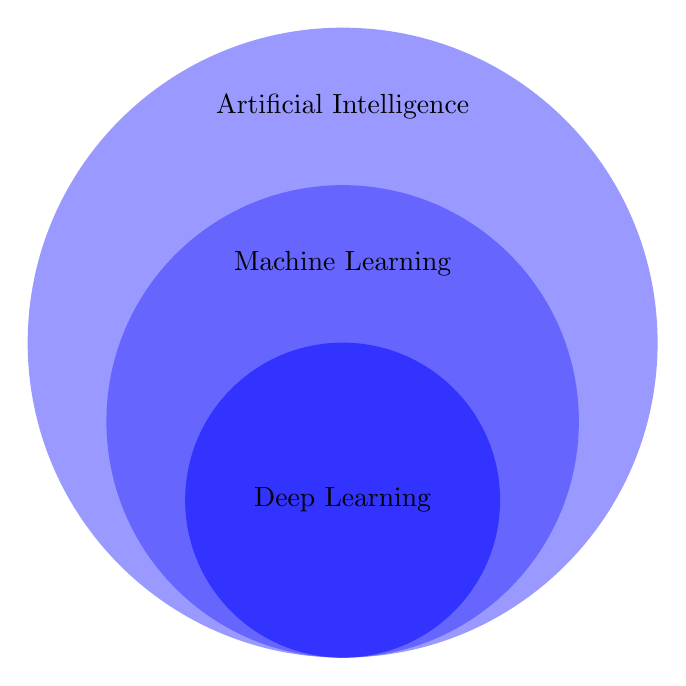
\begin{tikzpicture}
                \fill[blue!40!white] (5, 2) circle (4cm);
                \fill[blue!60!white] (5, 1) circle (3cm);
                \fill[blue!80!white] (5, 0) circle (2 cm);
                \node at (5,0) {Deep Learning};
                \node at (5,3) {Machine Learning};
                \node at (5, 5) {Artificial Intelligence};
                
            \end{tikzpicture}
        \end{center}

    \section{Links and References:}
        \subsection{Useful links:}
            \begin{itemize}
                \item \href{https://www.coursera.org/learn/machine-learning}{A Coursera/Stanford course on Machine Learning by Andrew Ng.}
                \item \href{https://www.coursera.org/specializations/deep-learning}{A Coursera/DeepLearning.ai specialization on Deep Learning.}
                \item \href{https://towardsdatascience.com/}{A blog on data science.}
                \item \href{http://incompleteideas.net/book/the-book-2nd.html}{A popular book on Reinforcement Learning.}
                \item \href{https://spinningup.openai.com/en/latest/}{A series on Deep Reinforcement Learning for video games.}
            \end{itemize}
        \subsection{Links to images and references:}
            \begin{itemize}
                \item \url{https://en.wikipedia.org/wiki/Artificial_intelligence}
                \item \url{https://en.wikipedia.org/wiki/Artificial_general_intelligence}
                \item \url{https://en.wikipedia.org/wiki/Machine_learning}
                \item \href{https://towardsdatascience.com/mnist-handwritten-digits-classification-using-a-convolutional-neural-network-cnn-af5fafbc35e9}{towardsdatascience.com}
                \item \url{https://commons.wikimedia.org/wiki/File:Detected-with-YOLO--Schreibtisch-mit-Objekten.jpg}
                \item \url{https://rapidapi.com/blog/top-facial-recognition-apis/}
                \item \url{https://medium.com/@amarbudhiraja/ml-101-linear-regression-tutorial-1e40e29f1934}
                \item \url{https://towardsdatascience.com/recurrent-neural-networks-d4642c9bc7ce}
                \item \url{https://medium.com/@awjuliani/on-solving-montezumas-revenge-2146d83f0bc3}
                \item \url{https://cps.iisc.ac.in/research/walking-robot/}s
            \end{itemize}

\end{document}
